\documentclass[10pt,a4paper]{article}
\usepackage[utf8]{inputenc}
\usepackage[T1]{fontenc}
\usepackage{lmodern}
\usepackage[margin=1.5cm, top=1.4cm, bottom=1.4cm]{geometry}
\usepackage{hyperref}
\usepackage{enumitem}
\usepackage{titlesec}
\usepackage{xcolor}
\usepackage{graphicx}

\definecolor{accent}{HTML}{00686E}
\hypersetup{colorlinks=true, urlcolor=accent, linkcolor=accent}
\pagenumbering{arabic}
\setlength{\parindent}{0pt}

\titleformat{\section}{\large\bfseries\color{accent}}{}{0em}{}[\vspace{-0.6em}\rule{\textwidth}{0.8pt}]
\titlespacing{\section}{0pt}{7pt}{4pt}

\newcommand{\role}[4]{%
  \textbf{#1} \hfill \textbf{#2}\\[1pt]%
  \textit{#3} \hfill \textit{#4}\\[2pt]%
}
\setlist[itemize]{leftmargin=1.2em, itemsep=1.5pt, topsep=2pt, parsep=0pt}

\begin{document}

% ================= HEADER =================
\begin{minipage}[c]{0.80\textwidth}
  {\Huge\bfseries Prabhavit Gupta}\\[3pt]
  {\color{accent}\large Forward Deployed Engineer: Agentic Automations, Enterprise Integrations \& Workflows}\\[6pt]
  {\footnotesize +39 351 610 7807 ~$\vert$~
  \href{mailto:prabhavitg@gmail.com}{prabhavitg@gmail.com} ~$\vert$~
  \href{https://www.linkedin.com/in/prabhavit/}{linkedin.com/in/prabhavit} ~$\vert$~
  \href{https://github.com/prab-gupta}{github.com/prab-gupta} ~$\vert$~
  Venice, Italy}
\end{minipage}\hfill
\begin{minipage}[c]{0.18\textwidth}
  \raggedleft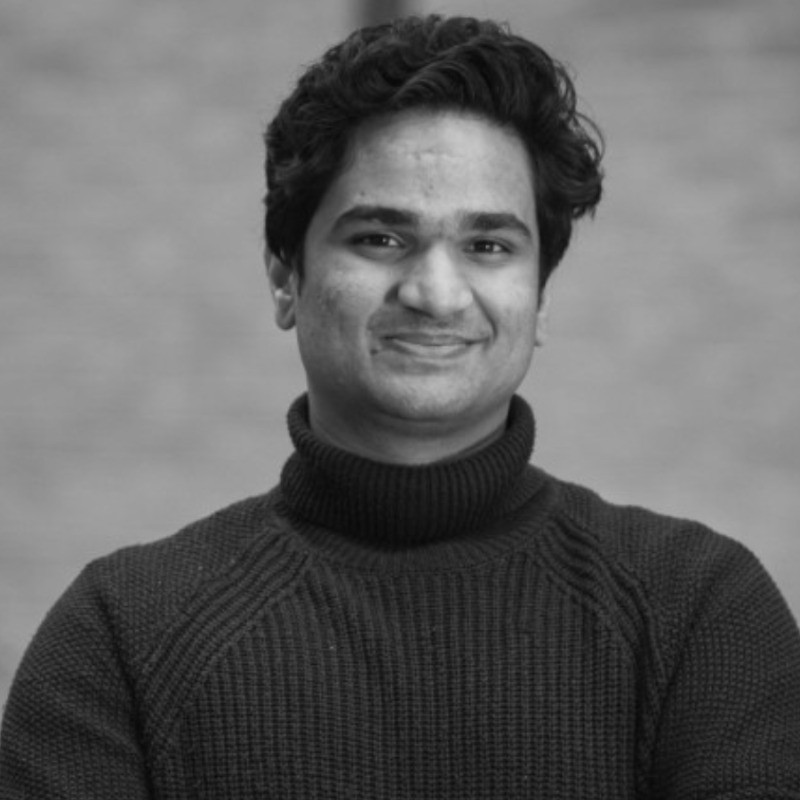
\includegraphics[width=2.0cm]{photo.jpg}
\end{minipage}
\vspace{-2pt}

% ================= SUMMARY =================
\section{Summary}
Forward Deployed Engineer and Automation Architect with 3 years of hands-on experience designing, building, and deploying mission-critical workflow automations, enterprise API integrations, and LLM-powered agent pipelines across European tech operations. Proven expertise embedding directly with business stakeholders and non-technical operators to translate undocumented, ambiguous processes into reliable, deterministic code and resilient automated workflows. Deep background in API integration (REST, webhooks, Supabase, third-party platforms), automated regression testing with Playwright, and LLM tool/function calling. Based in Venice, Italy with an EU Long Term Residence Permit (unrestricted EU work authorization without sponsorship). Immediately available.

% ================= TECHNICAL EXPERTISE =================
\section{Technical Expertise}
\begin{itemize}
  \item \textbf{Enterprise Automation \& Workflow Systems:} n8n, Workflow orchestration, Agentic systems, Exception handling architectures, Playwright end-to-end automations, Webhooks, Idempotent synchronization.
  \item \textbf{LLM \& Neurosymbolic Engineering:} LLM function calling, Tool use, Prompt engineering, Structured output extraction, RAG, Conversational interfaces, Knowledge ingestion pipelines.
  \item \textbf{Forward Deployed \& Solutions Engineering:} Technical discovery, Requirements scoping with business teams, Rapid POC delivery, Production troubleshooting, Enterprise onboarding.
  \item \textbf{Full Stack \& Integration APIs:} TypeScript, JavaScript, Node.js, Working-level Python, Next.js, React, RESTful APIs, Supabase, PostgreSQL, Docker, Git.
  \item \textbf{Languages \& Work Authorization:} Hindi (Native), English (C1 Professional), Italian (Beginner). EU Long Term Residence Permit (Permanent unrestricted EU work authorization; no visa sponsorship required).
\end{itemize}

% ================= EXPERIENCE =================
\section{Experience}

\role{\href{https://flowspace.co}{FlowSpace.co}}{Mar 2024 - Aug 2026}{Lead Developer (Full-time, Freelance)}{London, UK (remote)}
\begin{itemize}
  \item Directed full-stack platform architecture and integration engineering, embedding with commercial stakeholders to automate manual booking, billing, and inventory processes.
  \item Architected and deployed production customer support AI agents using LLM tool calling and live REST API function calling to query platform availability and execute bookings with deterministic safety checks.
  \item Resolved complex edge-case synchronization issues between external management systems (OfficeRnD, Nexudus) and internal databases using idempotent webhook reconciliation and automated exception handling.
  \item Built an automated knowledge ingestion pipeline: parsed heterogeneous unstructured documents (PDFs, spreadsheets, web pages) into structured database records, creating 900+ verified listings.
  \item Developed automated test harnesses and end-to-end validation suites with Playwright to verify customer-facing workflows and prevent regressions across multi-step integration paths.
  \item Served as the primary technical contact for enterprise B2B space partners, guiding onboarding, configuring API integrations, and troubleshooting production sync discrepancies.
  \item Scaled platform user base from 2,000 to 4,500+ active users through iterative product engineering and resilient frontend automations.
\end{itemize}

\role{Urlink}{Apr 2025 - Jul 2025}{Project Manager \& AI Assisted Developer (Freelance)}{Barcelona, Spain (remote)}
\begin{itemize}
  \item Led technical delivery of AI-assisted web applications, coordinating API contracts, database schemas, and external service integrations.
  \item Evaluated commercial LLM APIs across task types, optimizing prompt structures, schema adherence, and model selection for latency and output consistency.
  \item Implemented automated CI/CD checks and validation suites, ensuring clean code releases and minimal deployment regressions.
\end{itemize}

\role{Independent Technical Consultant}{Aug 2023 - Feb 2024}{AI Solutions \& Automation Engineer}{Venice, Italy}
\begin{itemize}
  \item Developed custom web automations, integration prototypes, and data extraction pipelines for European SME clients using TypeScript, Playwright, and APIs.
  \item Partnered directly with non-technical business founders to analyze operational bottlenecks, translating manual paper and spreadsheet workflows into automated software solutions.
  \item Implemented webhook listeners and data synchronization flows, replacing manual administrative processes and improving data accuracy.
\end{itemize}

% ================= EDUCATION =================
\section{Education}
\role{Ca' Foscari University of Venice}{2020 - 2024}{BA in Philosophy, International Studies and Economics}{Venice, Italy}
\begin{itemize}
  \item In-depth focus on formal logic, analytical problem solving, systems analysis, and macroeconomic decision models.
\end{itemize}

\end{document}
